\begin{quote}
"I have not failed. I've just found 10,000 ways that won't work." \\
\hspace*{\fill} — Thomas A. Edison
\end{quote}

Ah, the last milestone. Now that we have the ability to spawn an additional core, the goal of this milestone was to implement a full inter-core messaging and RPC system by extending our work from M4. We were fairly confident in our conceptual understanding of URPC, but faced several technical and non-technical challenges and we eventually ran out of time before we could implement a working solution. We try to describe our idea, what worked, and what didn't work in this final chapter.

\subsubsection*{The Idea} \label{sec:the_idea}
The idea behind this milestone was to take advantage of shared memory and cache coherency to implement a really fast messaging system between cores. While sharing memory is great when it comes to performance, we had to be extra careful in how we were handling reading/writing to shared memory given Barrelfish's weak memory consistency model. In particular, this meant our ring-buffer implementation had to make use of memory barriers to ensure that messages were written and read in the correct order. \autoref{figure:rough_idea} summarizes at a high-level how we envisoned M6 to work. A newly booted core receives a capability to a frame of with a size of two pages. One of these pages serves as the ring-buffer that this core will use to send messages, and the other half of the frame is used to receive messages. We will refer to these as the \textit{producer} page and the \textit{consumer} page going forward. Also, notice that arbitrary processes in each core cannot access the UMP prdoucer buffers directly. Instead, they must first send a LMP message to the \verb|init| process, which would then serve as the "messager" between that process and the other core. Keep this in mind since this was a major pain point for us that we discuss \hyperref[hurdles]{later}.

Since there was no LMP-like event-driven abstraction for UMP messages, we decided to spawn a thread in the \verb|init| process for each core dedicated to polling the consumer ring-buffer for messages and handling them appropriately. This is where we uncovered critical, blocking issues in our work from the previous milestones...

\subsubsection*{Hurdles} \label{sec:hurdles}
We realized that we were unable to spawn threads! Any attempt at using Barrelfish's threading library immediately resulted in kernel panics and ugly red error messages polluting our logs. We will save you the details but the issue was that we never tested for threading in the earlier milestones and did not consider thread safety of our systems until towards the end of the course. Moreover, we (wrongly) believed that paging didn't need to be thread-safe since processes would only access the paging interface via \verb|malloc| and friends - which are inherently thread-safe. We failed to consider the fact that the page fault handler and the process spawning methods heavily rely on the raw paging interface. Therefore, paging did, in fact, need to be thread-safe. We went ahead and made the slab/slot allocators thread-safe as well, just to be safe. 

Just to go back to the point on testing -- we believe we didn't write nearly enough tests across milestones, even though we knew better and always kept mentioning "we should write more tests". We attribute this to poor communication and distribution of tasks and the fact that we fell a little behind on the later milestones.

Initially, we tried to work around our threading issues by spawning a new UMP monitoring process on each core. This could have worked, but this meant that we would have to send an additional LMP message between this process and \verb|init| -- we felt this defeated the purpose of having fast shared-memory-based messaging since we would end up incurring an unnecessary context-switch cost.

Once we finally got threading working, we faced another issue with our M4 implementation -- we never considered the case where the \verb|init| process might want to push a message to a child process. Therefore, we were only able to achieve inter-core communication between the \verb|init| processes of two cores.
\subsubsection*{What Worked}
Clearly, not a lot was going our way in this milestone, but not all was lost! Our RPC message handlers from M4 were fairly decoupled from the underlying transport protocols and not a lot needed to be rewritten to implement the URPC message handlers. Moreover, we were able to use the idea of sharing memory to make M4 faster when it came to sharing arbitrary sized messages. We are also proud of the effort we put in in trying to get M6 to work -- a lot of sleep was sacrificed! But more importantly, we had fun and enjoyed every minute of time spent on this course.

\begin{figure}[h] 
	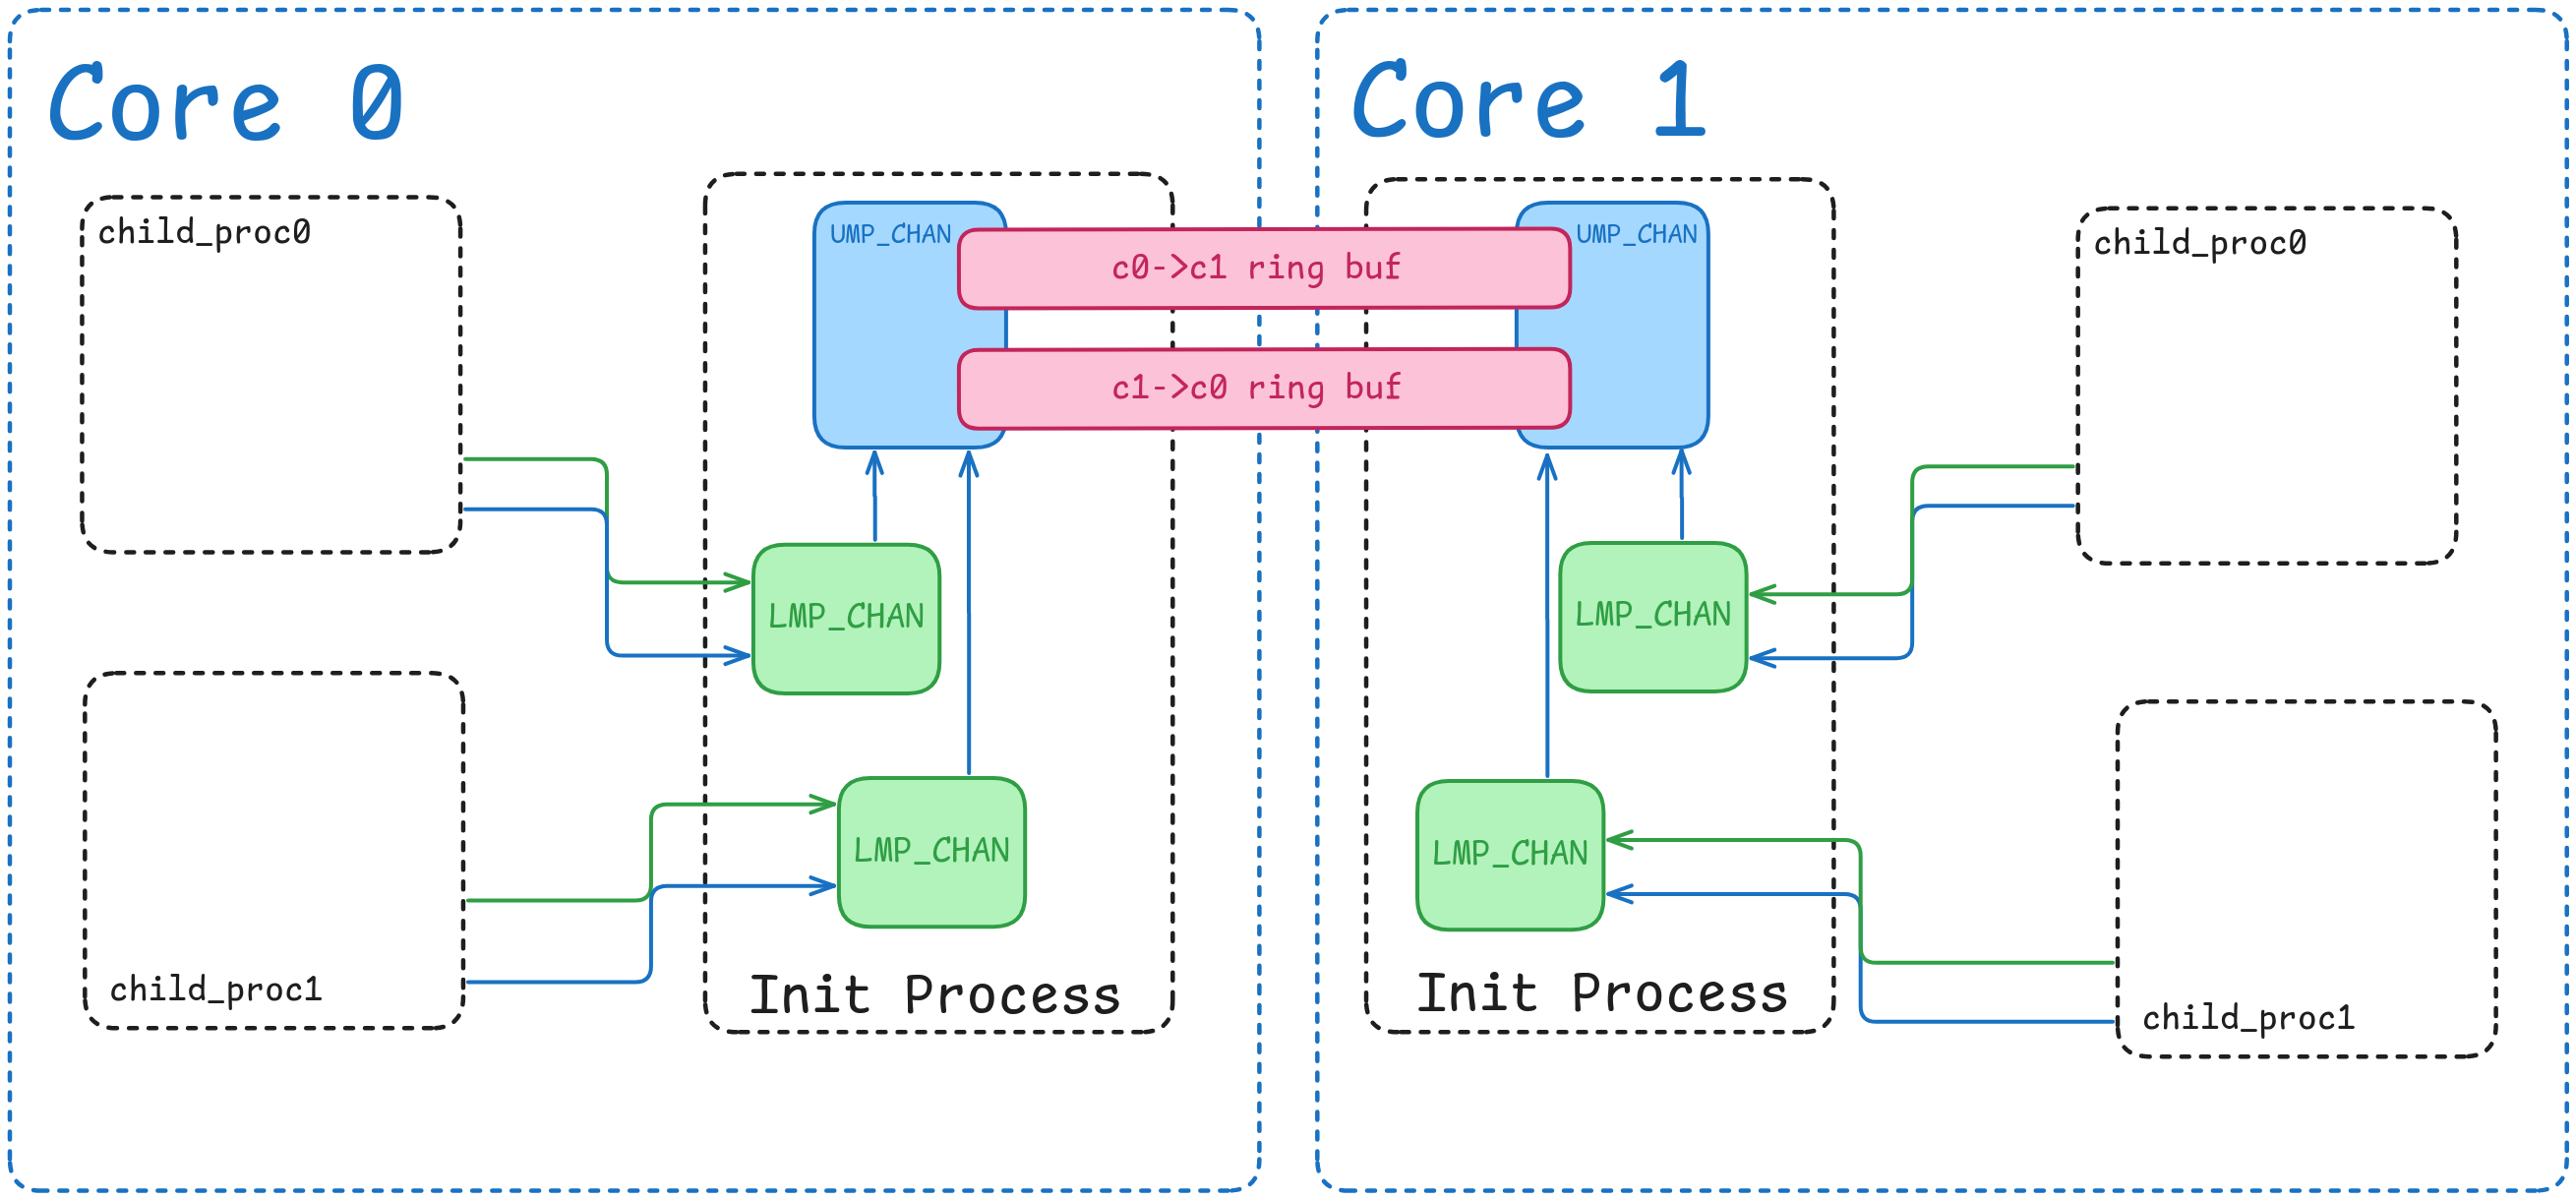
\includegraphics[width=\columnwidth]{report/images/rpc_lmp(3).png}
	\caption{A rough outline of our (intended) URPC system}
	\label{figure:rough_idea}
	\centering
\end{figure}
